\documentclass{article}
\usepackage[a4paper, portrait, margin=1in]{geometry}
\usepackage{amsmath, graphicx}
\graphicspath{{./images/}}
\usepackage[utf8]{inputenc}
\usepackage[english, macedonian]{babel}
\title{Мехатронички Системи: Управување со Повратна Врска}
\date{16/12/17}
\author{Галевски Марко 1172, Никола Мучев 1017, Елена Наумовска 1019}

\begin{document}
    \pagenumbering{gobble}
    \maketitle{}
    \newpage
    \pagenumbering{arabic}

\section{Вовед}
Роботика и автоматика стануваат потребни и основни делови од инженерството и следствено се многу важни теми за проучување од страна на студенти на инженерство и наука. Понатаму, роботика е изградена врз темели како карактеризација на трансдусери, контрола на мотори, собирање на податоци, механика на движење, мрежна комуникација, компјутерска перцепција, препознавање на шеми, кинематика, планирање на траекторија, и други кои исто така се темели за други полиња како на пример производство. National Instruments (NI) LabVIEW комплетот за роботика заедно со LabVIEW програмскиот пакет нудат додаток на традиционалните учебници за роботика, со можност за активно/практично учење во компактен и проширлив комплет.

Проектот беше изработен со цел да го прикаже концептот и принципот позади управувањето на некој систем со повратна врска. За остварувањето на задачата употребивме еден почетен кит за роботика од National Instruments, роботот DaNI 2.0. Овој роботски кит ги содржи сите компоненти потребни за успешна реализација на задачи и проекти поврзани со управувањето и задвижувањето на еден општ робот во форма на „Rover“. 

Во текот на овој документ ќе се разговара за структурата на роботот - односно неговите сензори и актуатори, како и за управувачката единица sbRIO, исто од NI. Потоа, ќе се претставаат и образложаат 3 алгоритми во LabVIEW. Првите два ќе бидат базирани на ПИД управување со повратна врска, додека третиот алгоритам ќе биде едно детално објаснување на почетната програмата дадена од NI како пример за можните способности на DaNI. За крај, ќе се продискутира за некои предизвици со кои се соочивме во текот на изработката на овој проект, и ќе се разговара за понатамошна работа со DaNI за постигнување на некоја корисна фунцкија.
\section{DaNI}

National Instruments (NI) LabVIEW комплетот за роботика го содржи DaNI: склопен робот со рамка, тркала, актуатори, сезори, sbRIO единица и кабли за поврзување. Хардверот може да биде проучуван, обратно инжениран, и модифициран од студенти. Меѓутоа, главната цел е роботска перцепција и контрола кои се имплементирани во LabVIEW софтвер развиен на одделен сервер (компјутер) и спуштен на роботскиот компјутер.

\begin{figure}[h]
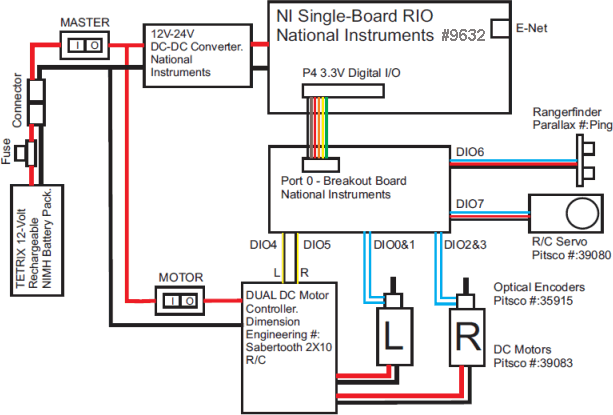
\includegraphics[width=0.75\linewidth]{dani_block_diagram.png}
\centering
\end{figure}

\subsection{Актуатори}
\subsubsection{DC Мотори}
\subsubsection{Серво Мотор}
\subsection{Сензори}
\subsubsection{Енкодер}
\subsubsection{Ултразвучен Сензор}

\section{NI sbRIO 9632}

\begin{figure}[h]
\includegraphics[width=0.75\linewidth]{sb_rio_1.png}
\centering
\end{figure}
sbRIO (single-board Reconfigurable Input/Output) управувачките единици од National Instruments претставуваат компјутер монитран на една плочка (single board) наменета за случаи каде што е потребно решение со управување во реално време (Real Time). Оперативен систем кој работи во реално време (RTOS: Real Time Operating System) е изработен со особената цел да извршува функции кои барат големо ниво на временска прецизност и висок степен на надежност. За некој систем да се смета за RTOS, тој мора да има познато максимално време на извршување за секоја од неговите клучни операции. Системите кои можат сигурно да обезбедат максимален временски одѕив се вели дека работаат во потполно реално време, додека системите кои можат само понекогаш да обезбедат максимален временски одѕив се вели дека работаат во делумно реално време.  
 
Потребната брзина се постигнува со користењето на FPGA чип како процесорска единица (дали имаше и обичен процесор покрај него?)

sbRIO поседува 110 дигитални влезови/излези, 100 од кои се оспособени за PWM (Pulse Width Modulation), а 10 од кои се наменети за ниско-фреквентна намена. sbRIO поседува и 32 аналогни влезови, и 8 аналогни излези (ПРОВЕРИ ГИ БРЗИНИТЕ И ПРЕЦИЗНОСТИТЕ)

sbRIO содржи и 3 сериски „С“ портови за поврзувањето на надворешни модули од NI за проширување на можностите на sbRIO да опфатат и актуација и аквизиција на податоци.
\subsection{PWM}

\subsection{FPGA}
FPGA, или „Field Programmable Gate Array“, претставува репрограмибилно интегрално коло кој поседува голем број на програмибилни логични порти. Кај обичните микроконтролери, логиката за управување се пишува и компајлира од некои програмски јазик како C, BASIC или некој графички јазик како G (LabVIEW). Во текот на овој процес се сублимираат во процесорски наредби како ADD и MOV. Низата на можните наредби е единствена за секој микропроцесор. Кај FPGA колата, програмата не се сублимира на наредби, туку самата внатрешна архитектура на колото се подредува со електромагнетни полиња. Како резултат, се добива конфигурација на логични порти која ќе ја извршува задачата опишана во првобитната програма. Бидејќи FPGA нудат хардверско решение, нивното работење е често многу пати побрзо од работењето на обичните микроконтролери, но се подраги.  

FPGA колото што се наоѓа во sbRIO-то е моделот Xilinx Spartan 6, кој поседува 6 милиони репрограмибилни логични порти.
\subsection{Споредба со Arduino Uno}

\section{LabVIEW}
LabVIEW (Laboratory Virtual Instrument Engineering Workbench) е софтверски пакет наменет за програмирањето на виртуелни уреди (инструменти) за мониторинг и управување на физички уреди. Инструментите што се програмираат во LabVIEW можат да се компајлираат и да се издават како комплетно независни програми кои можат да се монтираат како главен управувен софтвер на мехатроничките уреди и машини.  LabVIEW инструментите се програмираат користејќи го нивниот сопствен графички програмски јазик, „G“. Да се спомени дека јазикот G и G-Code немат никаква поврзаност меѓу себе.
Основниот пакет на LabVIEW поседува многу од стандардните можности што се очекуваат од било кој програмерски јазик, како што се логички/булови операции, математички операции, и пристап до алатки за визуелизација на податоци. 
LabVIEW може да се прошири (и во некои случаи мора да се прошири) со додатни пакети. На пример, овие пакети можат да содржат готови под-инструменти (sub-VIs) за обработка на сигнали (Signal Processing ), или да овозможуваат соработка помеѓу LabVIEW и некои други технологии (FPGA module). Од овие пакети ние ги употребуваме Real Time, FPGA, и Robotics пакетите. Првите два пакети ни го оспособуваат LabVIEW да програмира FPGA чипови и да управува во реално време, додека Robotics пакетот содржи во себе голем број на готови инструменти за обична и инверзна кинематика, отчитување од сензори, и праќање наредби на моторите. 
Robotics пакетот исто поседува едно подмножество на инструменти наменети само за DaNI 2.0, и со тие го управувавме DaNI роботот.  
\section{Управување со повратна врска}

\section{Предизвици}
\section{Заклучок}
\section{Понатамошна работа}


\end{document}
